% !TeX root = ../main.tex
\documentclass[./../main.tex]{subfiles}

\begin{document}

Với một trang web mang yếu tố nghệ thuật như web đọc truyện, bên cạnh nội dung nổi bật thì giao diện cũng đóng một vai trò vô cùng quan trọng trong trải nghiệm của người sử dụng. Phương châm thiết kế của Honyomi chính là sự đơn giản hóa trong giao diện mà vẫn truyền tải được đến người sử dụng những nội dung quan trọng của trang web.

\begin{figure}[H]
	\centering
	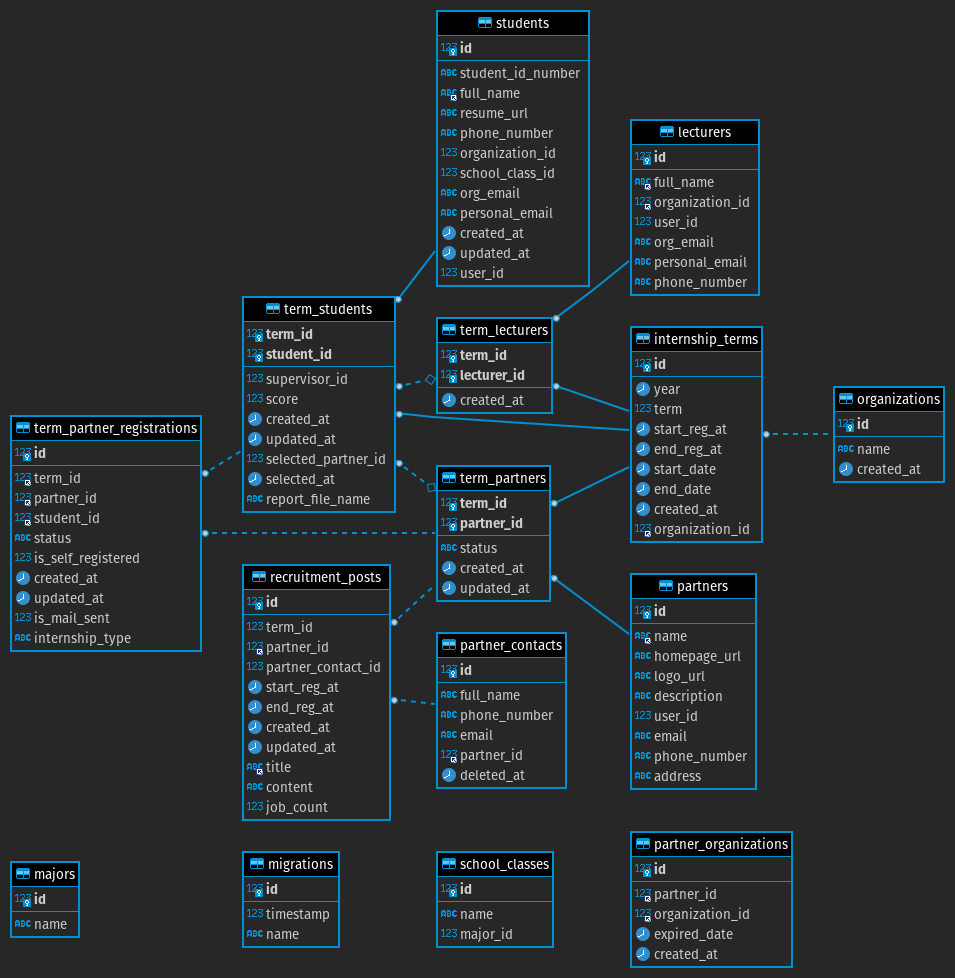
\includegraphics[width=\linewidth]{./images/image1.png}
	\caption{Luồng giao diện}
\end{figure}

\subsection{Màu sắc}

Honyomi có tông màu chủ đạo là 2 màu đen- trắng kết hợp với những mức độ đậm nhạt khác nhau, đem lại trải nghiệm đồng nhất cho toàn bộ trang web. Lý do Honyomi sử dụng tông màu này cũng vô cùng đơn giản:

\begin{itemize}
	\item Truyện tranh Nhật Bản thường được vẽ trên chất liệu đen trắng, vì thế Honyomi cũng muốn sử dụng 2 màu này để trang web trở nên có tính liên kết hơn với nội dung của trang web đang cung cấp.
	\item Với 2 màu trắng đen, trang web dễ dàng có thể cung cấp sự tương phản một cách rõ ràng giữa những thành phần của giao diện, từ đó người sử dụng có thể dễ dàng nhận ra những điểm nhấn trong trang web. Ngoài ra các điểm nhấn còn có thể điểm xuyết bằng các màu sắc khác cũng dễ dàng thu hút được sự chú ý của người sử dụng.
	\item Hơn nữa các thành viên trong nhóm cũng rất hiểu cảm giác đọc truyện ở những môi trường thiếu ánh sáng (như ban đêm hay phòng tối) thì dark mode (chế độ tối) là vô cùng quan trọng. Việc sử dụng tông màu đen trắng kết hợp cùng hoạt ảnh chuyển đổi trạng thái giúp cho trải nghiệm chế độ tối của người dùng được đưa lên tầm cao mới. Khi chuyển đổi chế độ sáng và tối, các thành phần trên giao diện vẫn thể hiện rõ độ tương phản giữa các thành phần mà không mất đi sự hài hòa, tổng thể của trang web.
\end{itemize}

\begin{figure}[H]
	\centering
	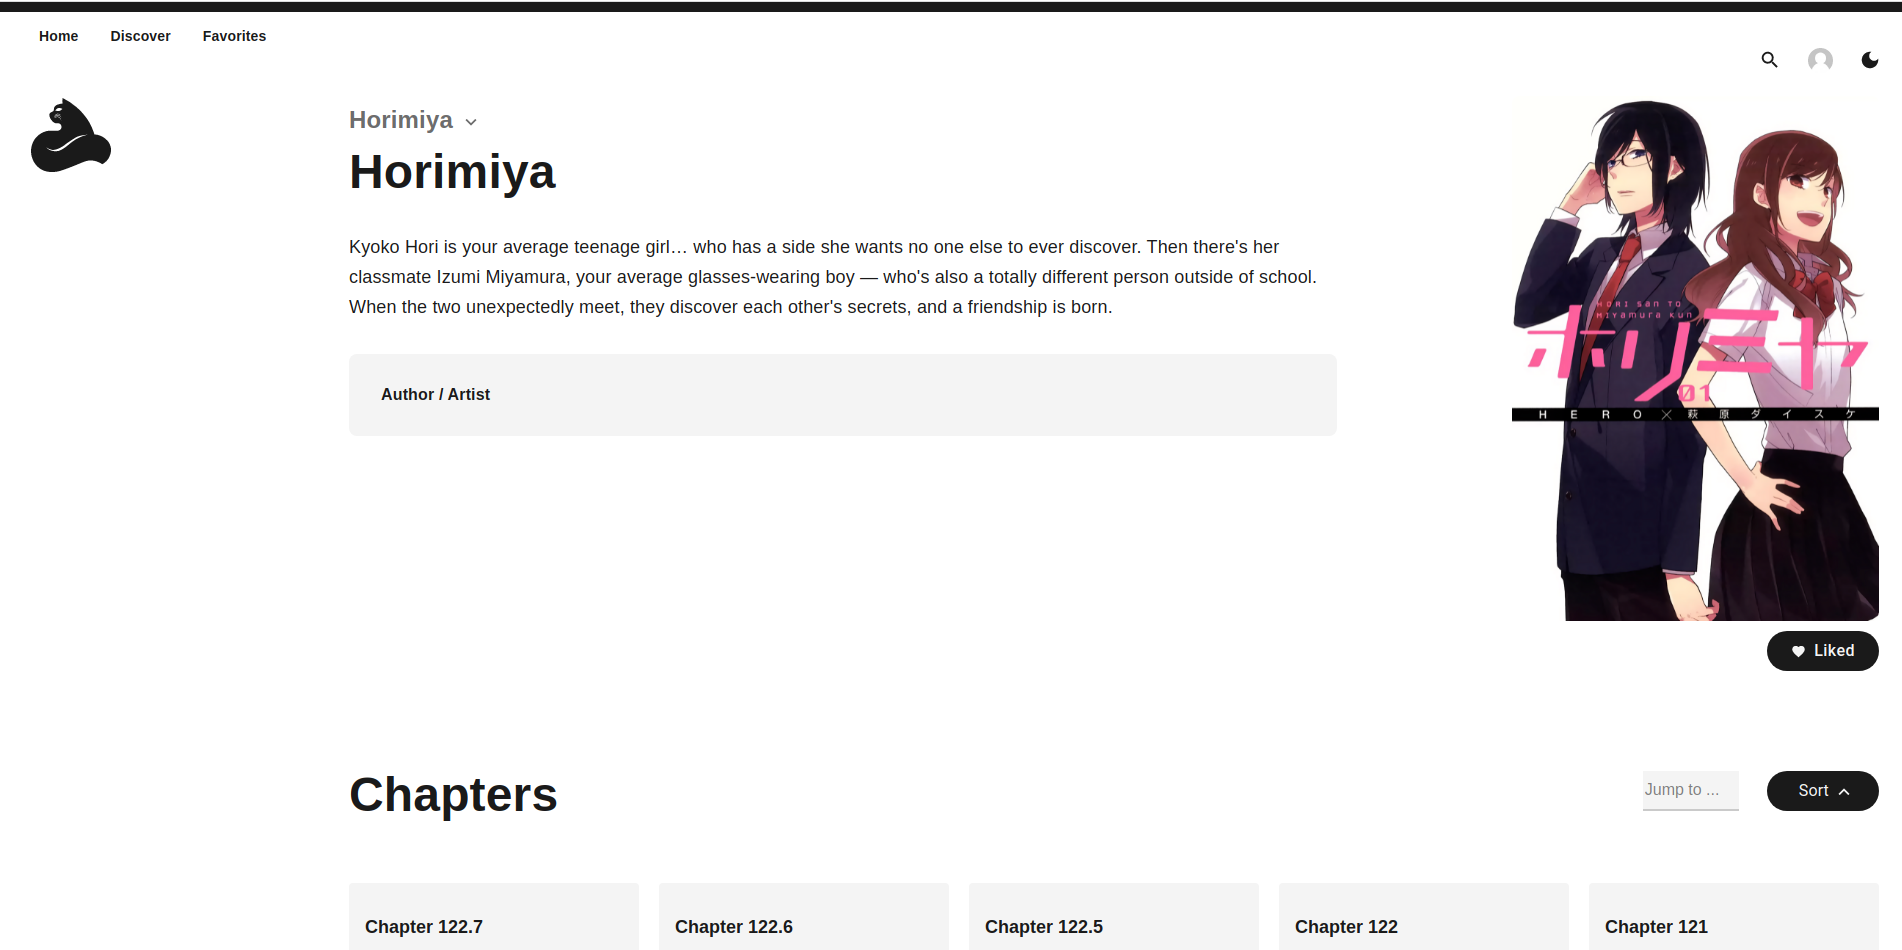
\includegraphics[width=\linewidth]{./images/image5.png}
	\caption{Màn hình giao diện sáng}
\end{figure}

\begin{figure}[H]
	\centering
	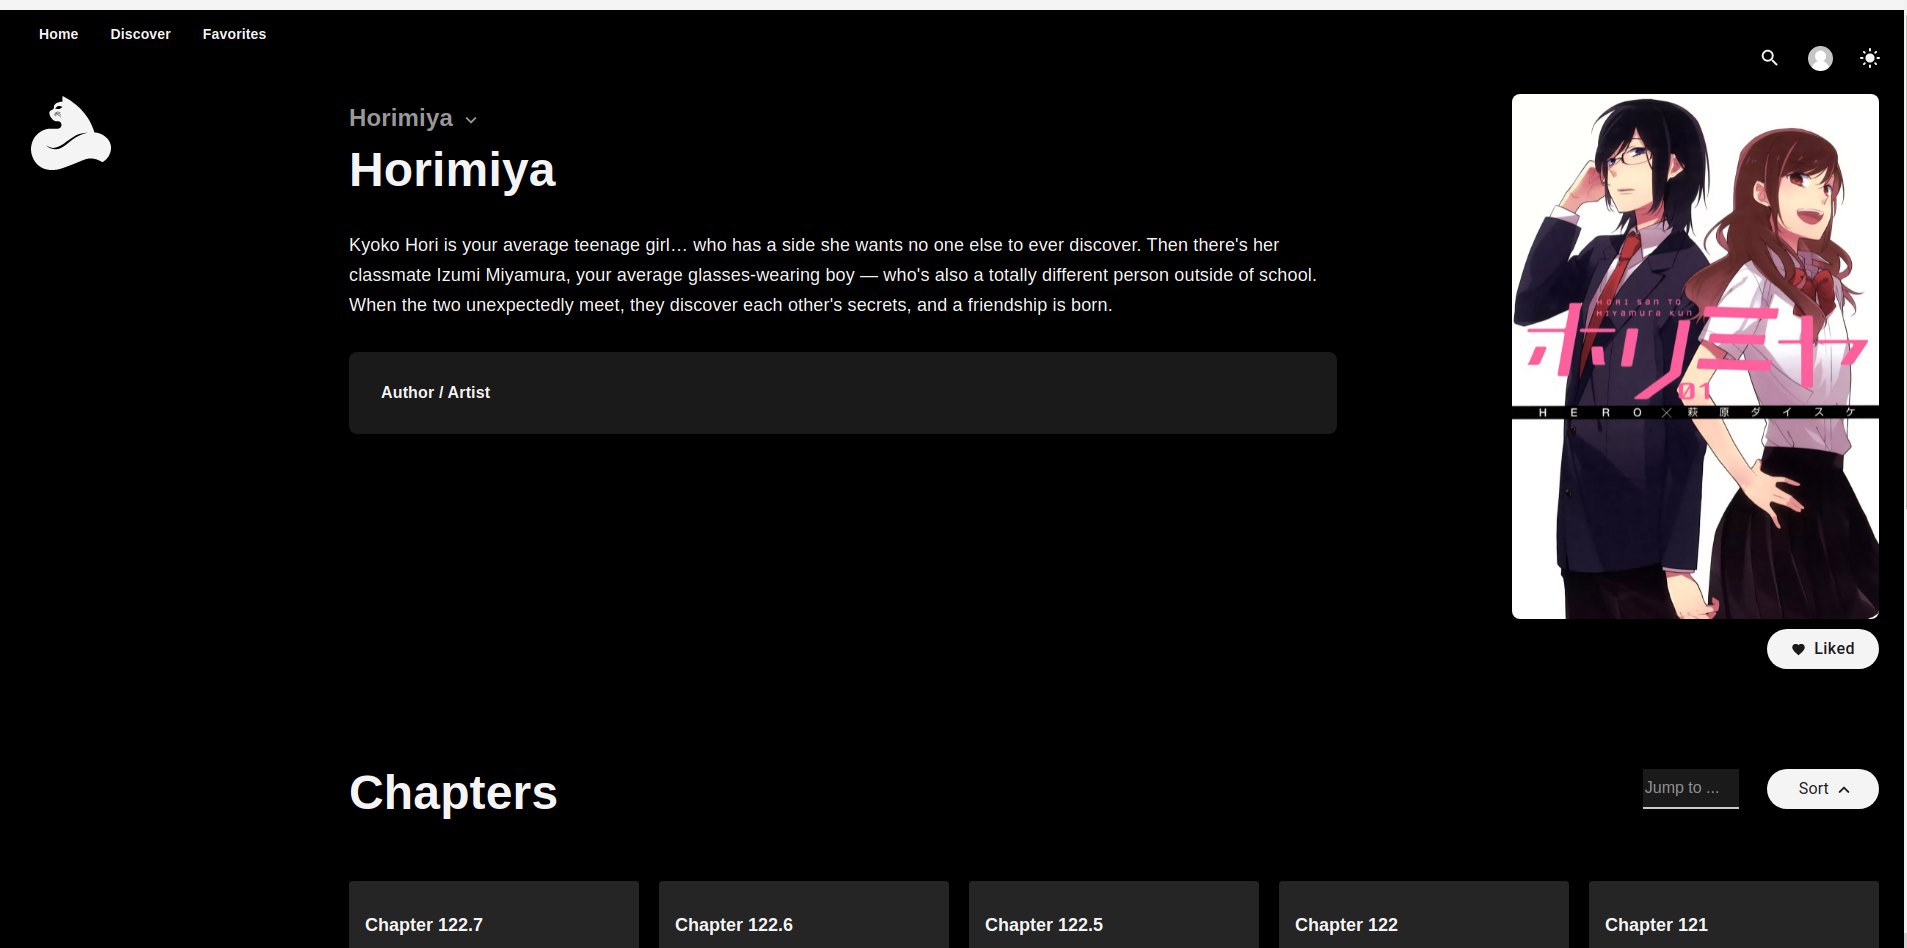
\includegraphics[width=\linewidth]{./images/image2.png}
	\caption{Màn hình giao diện tối}
\end{figure}

\subsection{Áp dụng các nguyên lý thiết kế}

Giao diện của các màn hình được thiết kế dựa theo 5 nguyên lý thiết kế giao diện người dùng: tính cân bằng (balanced), sự nhịp điệu (rhythm), sự hài hòa (harmony), sự thống trị (dominance), sự căn chỉnh (alignment).

Tính cân bằng và nhịp điệu được thể hiện thông qua việc phân chia giao diện thành các khối, sắp xếp vị trí của chúng cũng như các khoảng trống micro, macro một cách hợp lý và sau cùng là lặp lại đều đặn các phần tử có cùng chức năng.

\begin{figure}[H]
	\centering
	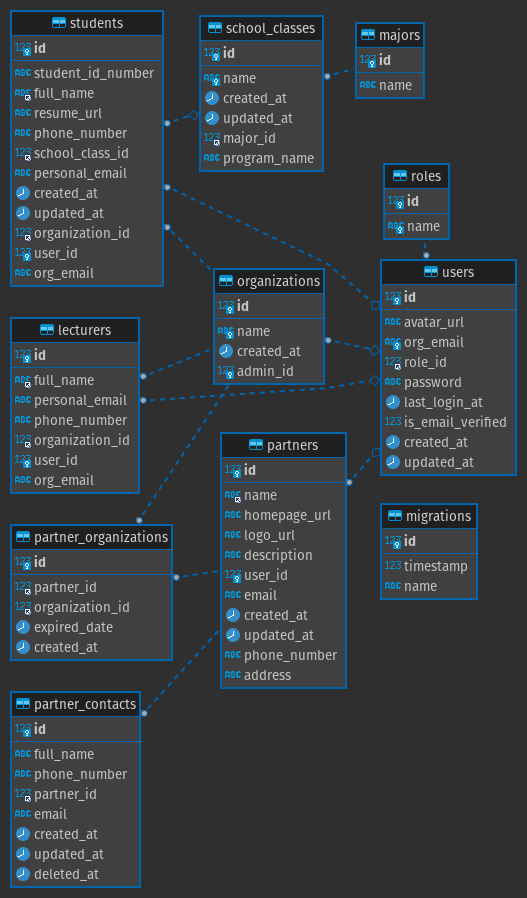
\includegraphics[width=\linewidth]{./images/image3.png}
	\caption{Áp dụng nguyên lý balance và rhythm}
\end{figure}

Đôi khi việc lặp đi lặp lại các phần tử sẽ gây ra cảm giác nhàm chán, khiến người dùng không biết nên nhìn vào đâu khi truy cập trang web. Để hạn chế điều này thì việc áp dụng nguyên lý hài hòa và thống trị sẽ làm nổi bật dụng ý của trang web, dẫn dắt sự chú ý của người dùng đến với các phần tử cần chú ý. Ví dụ: Trong màn hình trang chủ dưới đây, phần carousel nằm ở phía trên, chiếm nửa màn hình, có hình ảnh khá nổi bật chiếm ngay lấy sự chú ý của người dùng, từ đó hướng sự chú ý sang phần tên truyện được gợi ý khá to và đậm phía bên trái, cuối cùng là tới một nút bấm nổi bật với màu sắc tương phản dẫn tới trang đọc truyện.

\begin{figure}[H]
	\centering
	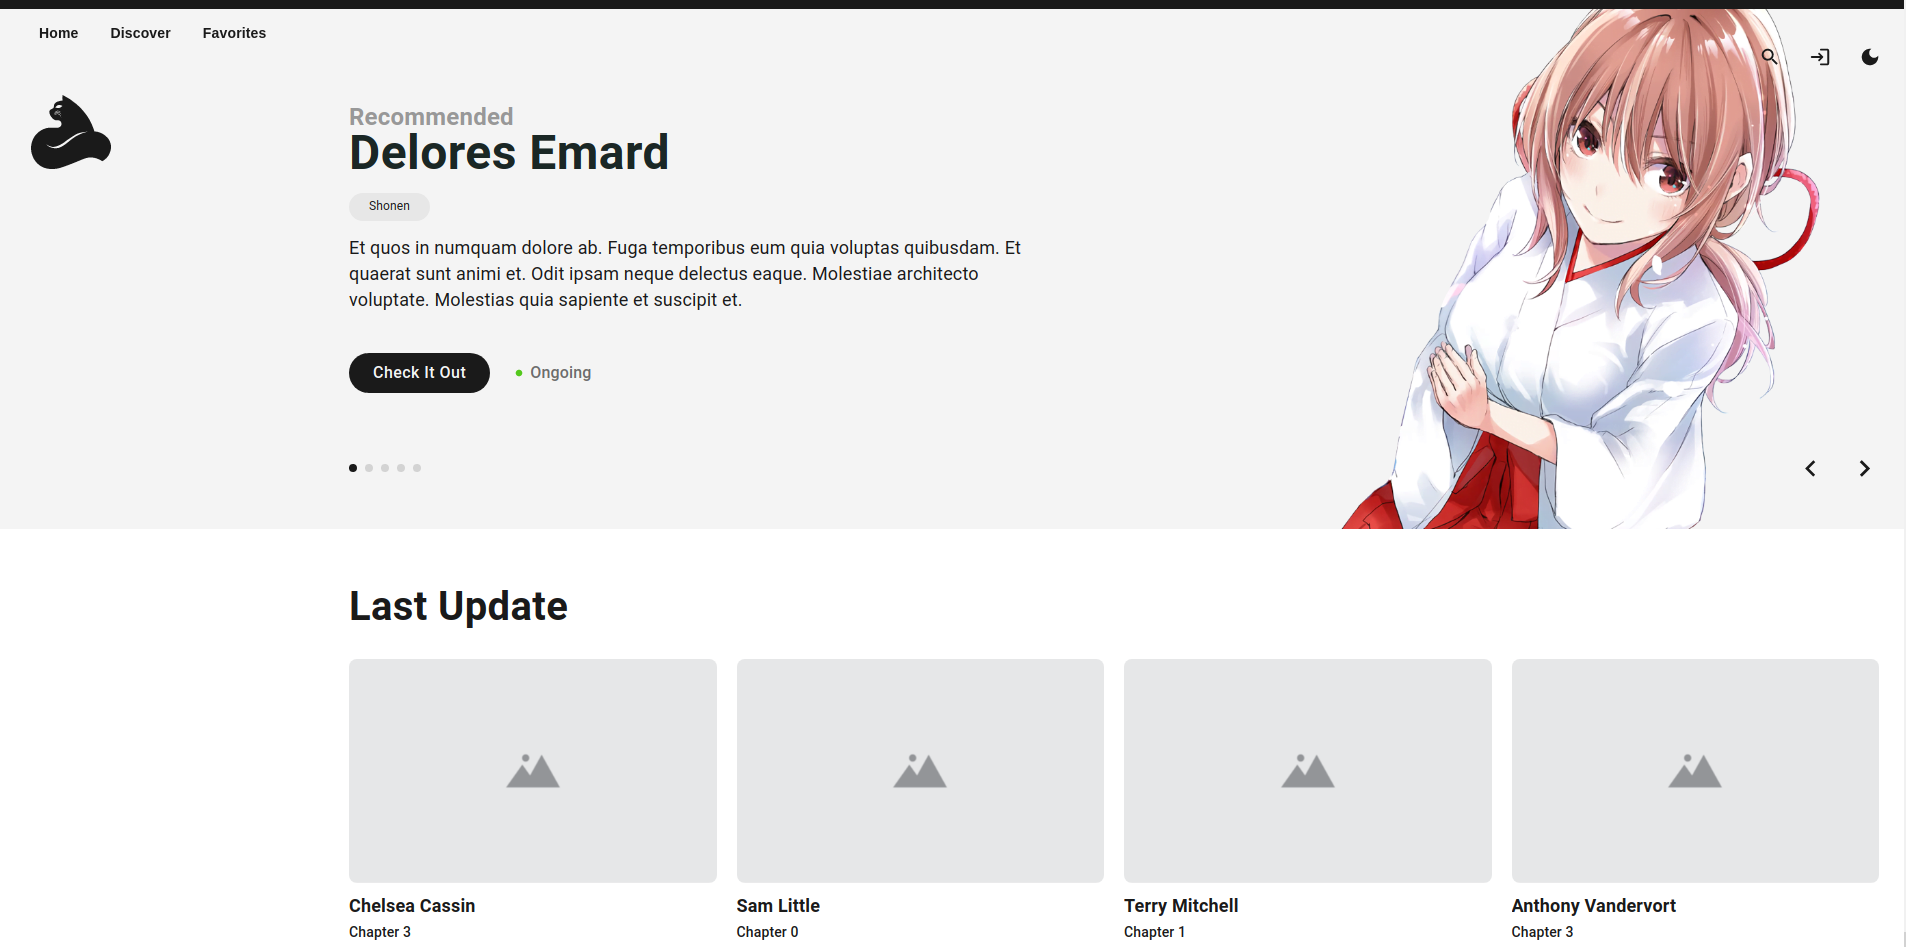
\includegraphics[width=\linewidth]{./images/image10.png}
	\caption{Áp dụng nguyên lý harmony và domindomi}
\end{figure}

Bố cục trang web của nhóm đều được căn chỉnh theo hệ thống lưới, làm mọi thứ trở nên ngay ngắn, có thứ tự, truyền tải sự hài hòa, giúp cho người dùng dễ dàng đọc và nắm bắt thông tin nhanh hơn. Ví dụ màn hình khám phá:

\begin{figure}[H]
	\centering
	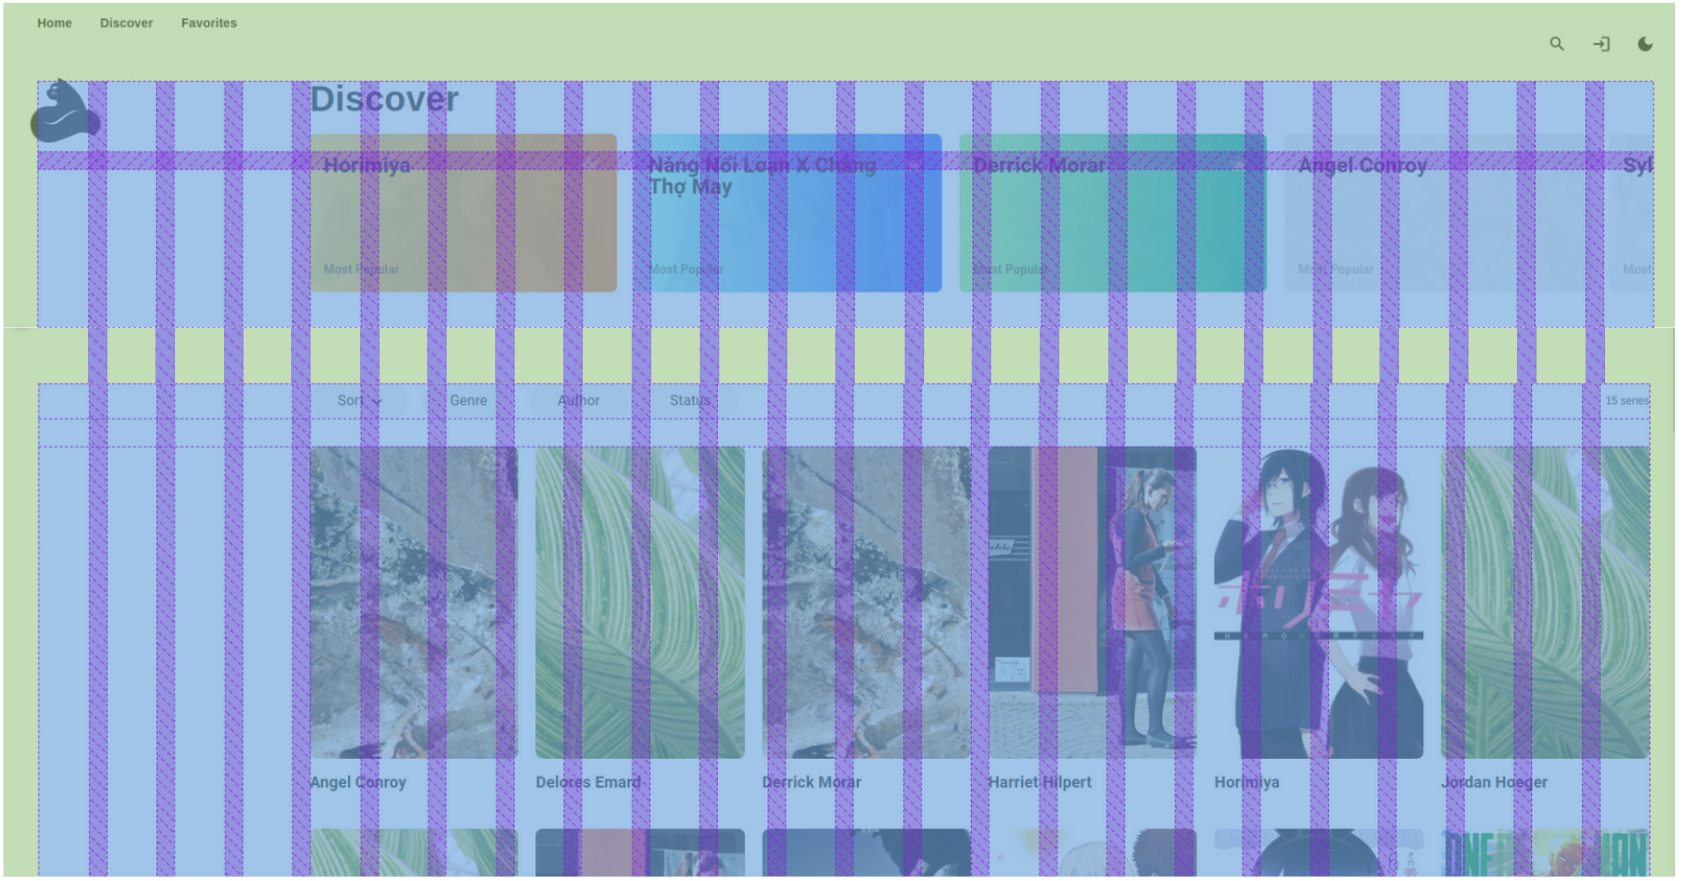
\includegraphics[width=\linewidth]{./images/image9.png}
	\caption{Áp dụng nguyên lý alignment}
\end{figure}

\end{document}